\ifdefined\THESIS
    \chapter{\uppercase{Location Prediction}}
\else
    \section{Location Prediction}
\fi

Based on the questions we answered in the previous section, we have enough
information to build a system for location prediction, which we call
FriendlyLocation.
Since the location prediction system will be run on a large number of users,
it must be fast and scalable.

\section{Edge Length Prediction}

We need to seperate the best contacts, who are likely to be nearby, from
bad contacts who are likely to be far away.
%
The factors that we investigated in the previous section indicate when someone
is likely to be nearby, but they don't guarantee it.
%
There are pairs of users who are reciprocal friends with a small number of
followers, a high local friend ratio, have conversations, and still live on
opposite sides of the globe.
%
Another problem with this data is that some of these factors are correlated
with each other; users with lots of followers tend to have a low friend contact
ratio.
%
Finally, celebrity accounts may be useless for determining which city a person
is from, but they might still suggest the user's home continent.

In \cite{backstrom2010find}, the authors present a model of the relationship
between distance and friendship that treats all of the edges the same.
%
We can improve the accuracy of this model by weighting some edges more strongly
than others.
%
We have several pieces of information, and want to map it to a single, extremely
noisy value: the distance to a contact.
%
This could be looked at as a classification problem where you want to classify
edges as local or non-local, but the problem is there is a smooth continuum
from local to non-local, and semi-local friends can be useful for location
prediction.
%
As a result, we model this as a regression problem.
%
Since most of the input features are correlated and either binary or non-linear,
linear regression is unlikely to work well.
%
\emph{more on why not other regression models?}
%
We chose to use a decision tree regressor based on the CART algorithm
(classification and regression trees) to distiguish the best edges from the
worst.
%
A decsision tree regressor works similiar to the well-known decision tree
classifier, except that it produces real numbers as output instead of discrete
classes.
%
During training, the training data is recursivly split based on the input
variable with the most predictive power to build a binary tree.
%
Each of the internal nodes of this tree have a cutoff for one of the input
variables, and the leaves of the tree have a predicted value.
%
\emph{Does this need a better explaination? Can we assume people know decision
trees?}

The regression tree was trained on several of the features from the previous
section that are correlated with users living near each other:
\begin{itemize}
\item the type of contact
\item if the target mentioned the contact
\item if the contact mentioned the target
\item if the contact had a protected account
\item the contact's follower and friend count
\item the PLE of the contact's location
\item the contact's local friend ratio
\end{itemize}
%
Since the distances between users varied by several orders of magnitude, we
trained the regressor to predict the log of the distance.
%
The tree regressor was configured to not split leafs with fewer than 1000 data
points to prevent over-fitting.
%
The predictor does not do a great job of predicting the actual distance to a
contact; there's simply too much noise.
%
However, it does do an excelent job of seperating the closest pairs of users
from the most distant pairs as we will show in the next section.


\section{Model}
\label{sec:model}

In this section, we build a model for the probability that a user, who we refer
%
to as the target user, lives at a specific location given the approximate
location of his contacts.
%
In the previous sections, we looked at the probability that a contact lives a
certain distance from a given user.
%
Location prediction requires the probability that the user lives at a specific
location.
%
We can find that by comparing the distribution of Twitter users to the various
types of contacts.


First, we needed a model for the density of Twitter users.
%
We calculate the distance between every target user and every contact
(even for contacts and users who had no relationship).
%
In order to speed up this calculation, we divide the world into a \.1 degree
by \.1 degree grid, and count the number of of contacts in each of the spots
on the grid.
%
We took the distances between users and sorted them into 360 logarithmically
scaled bins between 10 miles and 10,000 miles.
%
(Every edge less than 10 miles was ignored because it was around the size of
the grid boxes, and therefore, noisy. Distances greater than 10,000 miles are
on the opposite side of the world.)
%
We fit this segment to a power law curve, which gives us a way to estimate
$\stgrEdges$.

Next, we need to model the probability that two users are contacts.
%
We ran the decsision tree regressor on the training data to create a set of
tuples $T = (d_i, p_i)$ for $d_i \in D$ and $p_i \in P$ where $d_i$ is the
actual length of the edge, and $p_i$ is the value predicted by the decision
tree.
%
We split $T$ into $k$ quantiles on the boundaries $\{q_0,\cdots,q_k\}$ as
follows:

\[
    q_i =
    \begin{cases}
        P_{(1+\lfloor i|T|/k \rfloor)}, & i=<k \\
        \infty & i=k
    \end{cases}
\]

We split the edges in these groups into 480 logarithmically-scaled bins from 1
to 10,000 miles based on the length of the edge.
%
We divided the number of edges that actually existed at each distance by the
number of edges that could have existed as predicted by $\stgrEdges$.

\[
\pContact{_i}(dist) = \frac{\nebrEdges{_i}(dist)}{\stgrEdges(dist)}
\]


We fit $pContact$ to the curve from \cite{backstrom2010find}:
\[
    \pContact{_i}(dist) = a_{i} \times (b_{i}+dist)^{-c_{i}}
\]


\begin{figure}[tbh]
\centering
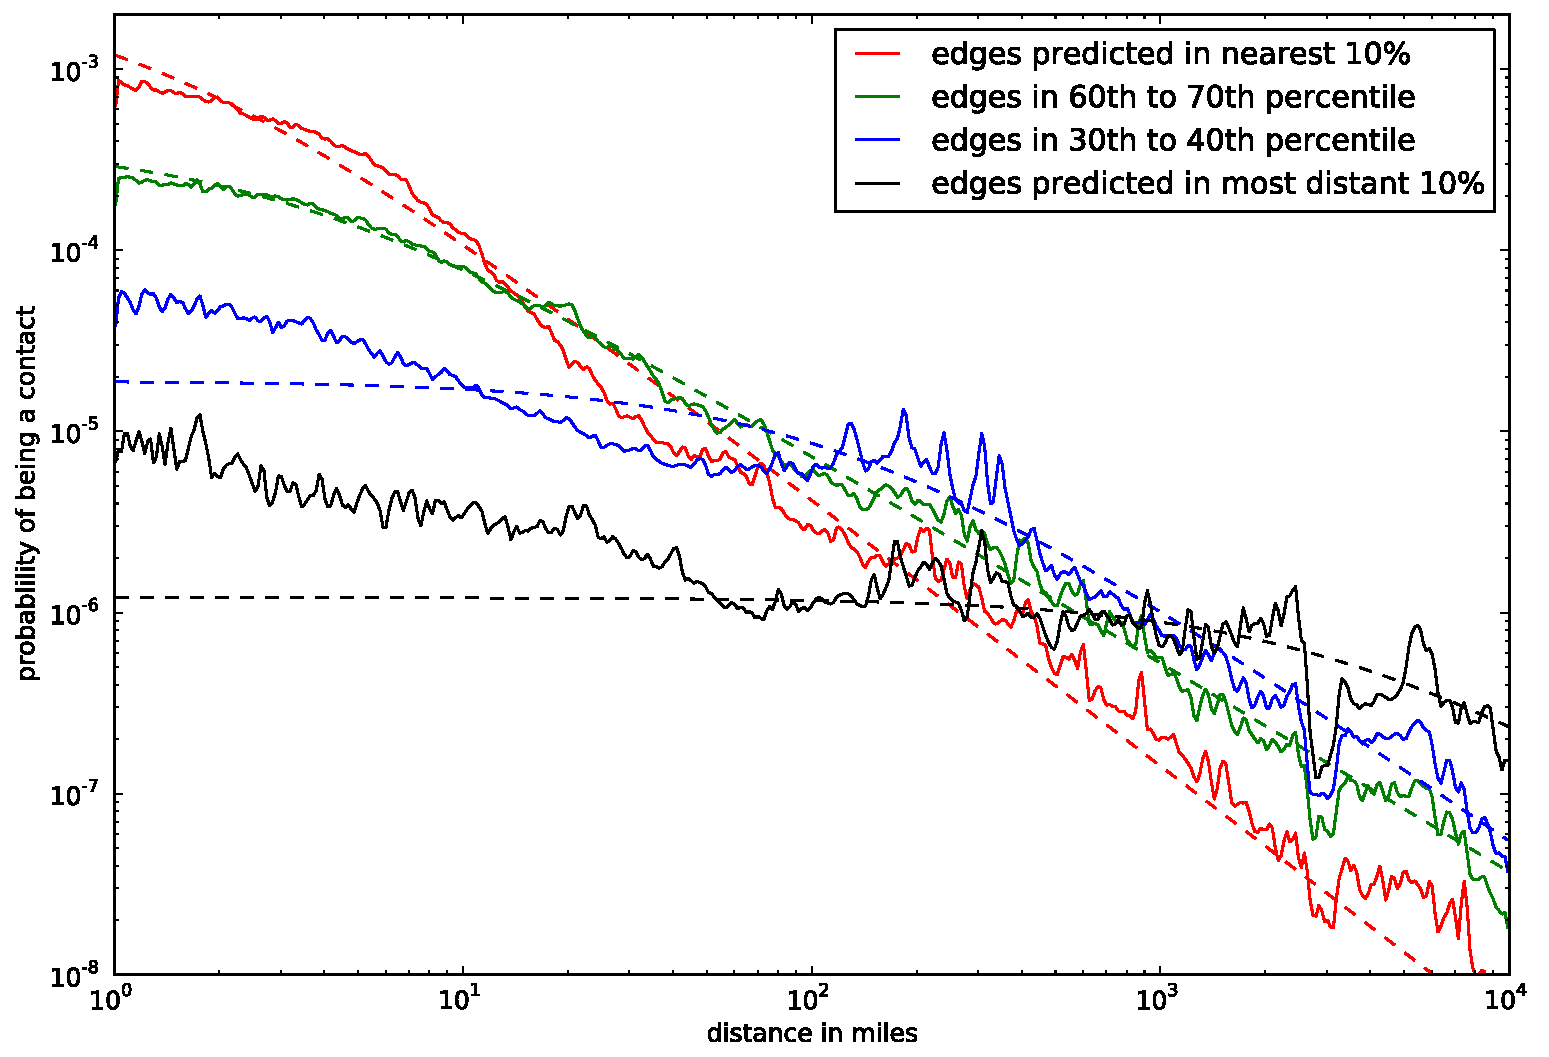
\includegraphics[width=\linewidth]{figures/near_prob_fit.pdf}
\caption{
After splitting edges into groups based on their predicted distance, each group
was fit to a curve. Here are four of the ten curves and their curves of best
fit. The other six curves of best fit are shown as faint dotted lines. The
decision tree does a reasonable job of seperating the best edges from the worst
edges.
}
\label{fig:NearProbFit}
\end{figure}

This gave us 10 different curves for the probability that a certain type of
contact exists between a pair of users.
%
Four of the ten curves from one of the five evaluation groups and their lines
of best fit are shown in Figure~\ref{fig:NearProbFit}.
%
The best contacts are orders of magnitude more
likely to live near a target user than the worst contacts.
%
If the predictions from the tree regressor were ignored, and users were placed
into one group instead of ten equal groups, this would reduce to the model
for friendship and distance presented in \cite{backstrom2010find}.


\section{System}
We used this model to build a Maximum Likelihood Estimator.

\[
    \MLELocation(L,P) = \argmax_{l_i \in L}
    \prod_{j=1}^{|L|} blah
\]

\begin{algorithm}
  %\label{alg:friendloc}
  \caption{FriendlyLocation \label{alg:friendloc}}
  \begin{algorithmic}[0]
  \Input{The contacts $contacts$}
  \Output{The predicted location}
  \State locations = list()
  \State predictedDists = list()
  \ForEach{contact \textbf{in} contacts}
      \If{contact.location \textbf{is} None}
        \State \Continue
      \EndIf
      \State locations.append(contact.location)
      \State dist = regressionTree.predict(contact.features)
      \State predictedDists.append(dist)
  \EndFor
  \State best = MLELocation(locations,predictedDists)
  \State \Return locations[best]
  \end{algorithmic}
\end{algorithm}

FIXME: formula for MLE, and description
FIXME: more here
FIXME: non-independent as seen in~\ref{sec:closer}

